\begin{figure}[t]
\centering
\resizebox{\textwidth}{!}{%
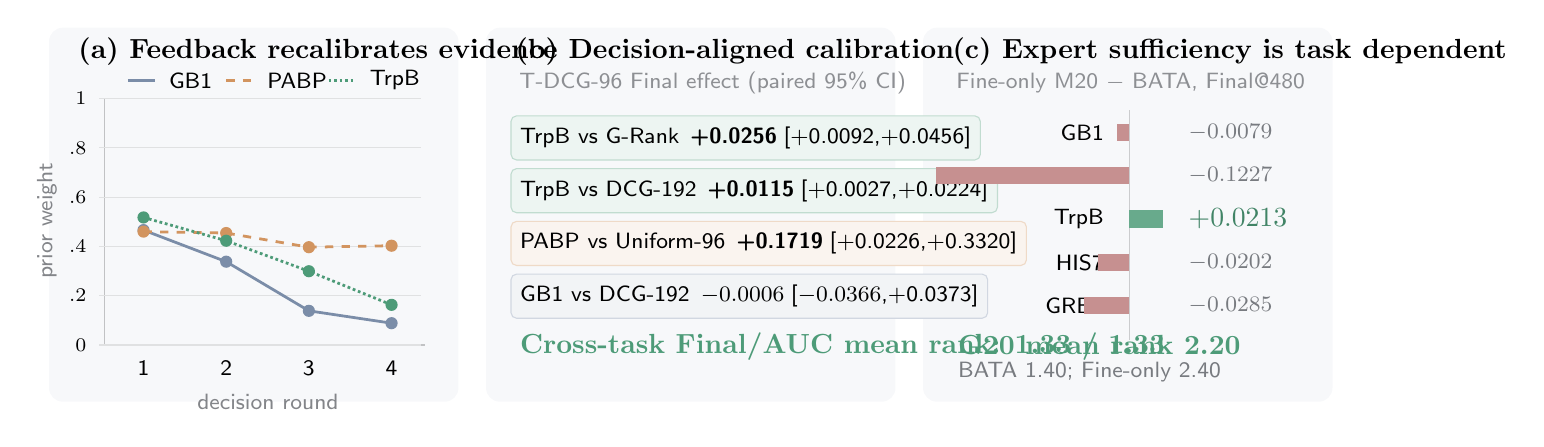
\begin{tikzpicture}[font=\sffamily\fontsize{8.1}{9.3}\selectfont]
\definecolor{gb}{HTML}{7B8DA8}\definecolor{pa}{HTML}{D2945F}\definecolor{tr}{HTML}{4D9B78}\definecolor{bata}{HTML}{4D9B78}\definecolor{neg}{HTML}{B36B6B}\definecolor{panel}{HTML}{F7F8FA}\definecolor{ink}{HTML}{30343B}
\foreach \x in {0,5.55,11.1}{\fill[panel,rounded corners=5pt] (\x,0) rectangle ++(5.2,4.75);}
\node[anchor=west,font=\bfseries] at (.25,4.45) {(a) Feedback recalibrates evidence};\draw[ink!30] (.70,.72)--(.70,3.85);\draw[ink!30] (.70,.72)--(4.78,.72);\foreach \r/\x in {1/1.20,2/2.25,3/3.30,4/4.35}{\node[anchor=north] at (\x,.64){\r};}\node[rotate=90,anchor=south,text=ink!60] at (.22,2.30){prior weight};\node[anchor=north,text=ink!60] at (2.78,.22){decision round};\foreach \v/\yy in {0/.72,.2/1.346,.4/1.972,.6/2.598,.8/3.224,1/3.85}{\draw[ink!15](.64,\yy)--(4.72,\yy);\node[anchor=east,font=\fontsize{6.8}{8}\selectfont] at (.60,\yy){\v};}
\draw[gb,line width=1pt](1.20,2.179)--(2.25,1.778)--(3.30,1.154)--(4.35,.997);\foreach \x/\y in {1.20/2.179,2.25/1.778,3.30/1.154,4.35/.997}{\fill[gb](\x,\y)circle(2.2pt);}\draw[pa,line width=1pt,dashed](1.20,2.160)--(2.25,2.142)--(3.30,1.962)--(4.35,1.981);\foreach \x/\y in {1.20/2.160,2.25/2.142,3.30/1.962,4.35/1.981}{\fill[pa](\x,\y)circle(2.2pt);}\draw[tr,line width=1pt,densely dotted](1.20,2.340)--(2.25,2.044)--(3.30,1.657)--(4.35,1.230);\foreach \x/\y in {1.20/2.340,2.25/2.044,3.30/1.657,4.35/1.230}{\fill[tr](\x,\y)circle(2.2pt);}\draw[gb,line width=1pt](1.0,4.08)--(1.35,4.08);\node[anchor=west] at (1.40,4.08){GB1};\draw[pa,line width=1pt,dashed](2.25,4.08)--(2.60,4.08);\node[anchor=west] at (2.65,4.08){PABP};\draw[tr,line width=1pt,densely dotted](3.55,4.08)--(3.90,4.08);\node[anchor=west] at (3.95,4.08){TrpB};
\node[anchor=west,font=\bfseries] at (5.80,4.45) {(b) Decision-aligned calibration};\node[anchor=west,text=ink!55] at (5.85,4.05){T-DCG-96 Final effect (paired 95\% CI)};
\node[anchor=west,rounded corners=2pt,fill=tr!10,draw=tr!35,minimum width=4.35cm,minimum height=.56cm,align=left] at (5.86,3.35){TrpB vs G-Rank\hspace{4pt}\textbf{+0.0256}\;[+0.0092,+0.0456]};
\node[anchor=west,rounded corners=2pt,fill=tr!10,draw=tr!35,minimum width=4.35cm,minimum height=.56cm,align=left] at (5.86,2.68){TrpB vs DCG-192\hspace{4pt}\textbf{+0.0115}\;[+0.0027,+0.0224]};
\node[anchor=west,rounded corners=2pt,fill=pa!10,draw=pa!35,minimum width=4.35cm,minimum height=.56cm,align=left] at (5.86,2.01){PABP vs Uniform-96\hspace{4pt}\textbf{+0.1719}\;[+0.0226,+0.3320]};
\node[anchor=west,rounded corners=2pt,fill=gb!10,draw=gb!35,minimum width=4.35cm,minimum height=.56cm,align=left] at (5.86,1.34){GB1 vs DCG-192\hspace{4pt}\textbf{$-0.0006$}\;[$-0.0366$,+0.0373]};
\node[anchor=west,text=bata,font=\bfseries] at (5.86,.70){Cross-task Final/AUC mean rank: 1.33 / 1.33};
\node[anchor=west,font=\bfseries] at (11.35,4.45) {(c) Expert sufficiency is task dependent};\node[anchor=west,text=ink!55] at (11.40,4.05){Fine-only M20 $-$ BATA, Final@480};\draw[ink!25](13.72,.78)--(13.72,3.70);\foreach \name/\y in {GB1/3.42,PABP/2.87,TrpB/2.32,HIS7/1.77,GRB2/1.22}{\node[anchor=east] at (13.52,\y){\name};}\fill[neg!75](13.562,3.31) rectangle (13.72,3.53);\node[anchor=west,text=ink!65] at (14.35,3.42){$-0.0079$};\fill[neg!75](11.266,2.76) rectangle (13.72,2.98);\node[anchor=west,text=ink!65] at (14.35,2.87){$-0.1227$};\fill[bata!85](13.72,2.21) rectangle (14.146,2.43);\node[anchor=west,text=bata!85!black,font=\bfseries] at (14.35,2.32){$+0.0213$};\fill[neg!75](13.316,1.66) rectangle (13.72,1.88);\node[anchor=west,text=ink!65] at (14.35,1.77){$-0.0202$};\fill[neg!75](13.150,1.11) rectangle (13.72,1.33);\node[anchor=west,text=ink!65] at (14.35,1.22){$-0.0285$};\node[anchor=west,font=\bfseries,text=bata] at (11.42,.72){G20 mean rank 2.20};\node[anchor=west,text=ink!65] at (11.42,.38){BATA 1.40; Fine-only 2.40};
\end{tikzpicture}}
\caption{\textbf{Mechanism analysis follows the paper's three questions.} (a) The prior-informed weight changes across rounds and differs by landscape, showing task-dependent feedback calibration. (b) Matched objective comparisons isolate decision alignment: tail weighting is supported on PABP and matching the calibration scale to the next batch is supported on TrpB, while GB1 shows similar top-96 and top-192 outcomes. (c) A stronger assay-only expert surpasses BATA on TrpB but not on the other four evaluated landscapes; a simple weight-threshold router does not improve the five-task mean rank. Full tables and confidence intervals are provided in the appendix.}
\label{fig:mechanism}
\end{figure}
